\chapter{Conclusion}
\graphicspath{{./Conclusion/img/}}

The current procedure often doesn't find a sign in many frames, the reason for that is the very high congruence and coverage
treshhold. When decreasing it, the signs are found more often, but there are also many false positives. False positives are
even worse than only finding a surface once in 100 frames. When a robot drives along a track or just 
straight forward in the direction of a sign. There are many different viewing angles and a lot of frames will pass the algorithm,
till it reaches a point, where it can't see the sign, there are a lot of chances to get a positive and true match. But if
using a lower minimum for the congruence a lot of false positives may occur, so a method has to be found to find out,
which one is a true and which one is a false result if gathering multiple different matches for a surface.
Unfortunately, in many cases there are a lot of false positives when allowing a congruence smaller than 87\%, so 
it will be impossible to obtain the right match for a sign with only analyzing the amount of finds.
A good possiblity would be, to track the object and then get the best match while seeing the object.
But unfortunately there was not enough time to implement such a piece of software in the end. 
Table \vref{table:RESULT} shows the settings which have proven to be suitable for each processing step.

\begin{table}[H]
	\centering
	\begin{tabular}{lcc}
		Process Step Setting 							   & Value                 & Unit \\
		Bluring Depth Map Size							   & 5\footnotemark[1]     & px   \\
		Bluring Angle Map Size							   & 16\footnotemark[1]    & px   \\
		Angle Filter (Z-Axis Min-Max)                      & 10-35                 & degrees \\
		Surface Width (Min-Max)                            & 20-200                & px \\
		Surface Height (Min-Max)                           & 20-200                & px \\
		Template Matching Congruence (Min)                 & 87                    & percent \\
		Template Matching Coverage (Min)                   & 70                    & percent \\
	\end{tabular}
\caption{Software Setting Results}
\label{table:RESULT}
\end{table}
\footnotetext[1]{Distance from the center pixel}

The most interesting aspect of this work, is the invention of the neighborhood map. The neighborhood map has been proven
to be a good ally in bluring and seperating surfaces from a depth image. There were no performance
measures for a comparison of the bilateral filter delivered by OpenCV and the bluring method in this work,
but when using the bilateral filter to blur the depth image, a instant drop in the frame rate of the depth image is visible
without measuring it, when using the cross blur filter mentioned here, this isn't the case. Currently the only lack
of the neighboorhood map are edges, which aren't created by a object infront of a background, like marked in figure \vref{figure:InnerEdges}.
The reason for the missing feature is, that it wasn't necessary, because only surfaces which look directly to the camera 
are interesting for sign recognition. For adding this feature a closer look at a gradient analysis of the depth image,
like it was done by Mr. Kühner in his bachelor thesis \cite{max:recog}, would be necessary.

\begin{figure}[H]
\begin{center}
  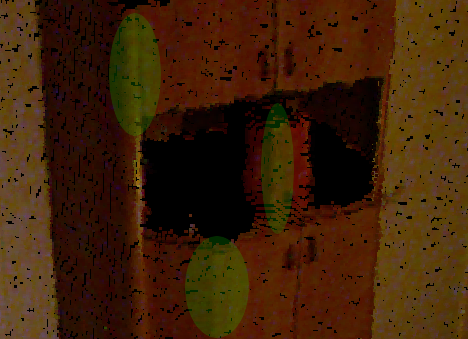
\includegraphics[width=\textwidth]{innerEdge.png}
  \caption{Inner-Object-Edges (marked green)}
  \label{figure:InnerEdges}
\end{center}
\end{figure}

Another interesting aspect is the template matching algorithm, which searches for proportions and resizes the
template to the appropriate size. The advantage of this algorithm is clearly, that a image has to be passed
only once for finding suitable proportions and the template will be scaled properly, making it possible
to find matches in a huge range of different scalings. In a normal template matching algorithm,
this would mean, to shift a template all over the picture and compare it at any place and scaling.
The performance needed for an algorithm doing that, would be really enormous.
of time for processing. A disadvantage of this template matching functionality is that it will not
find the template inside of a picture when the surface is rotated, but in this work, this is
is fixed by using the real world coordinates to warp the perspective, so the target pattern
will be visible at the right proportions. But unfortunately there's another disadvantage,
if the camera is rotated a few degrees, the alogrithm will not find the picture anymore.
A approach to this problem could be to try to read out the accelerometer of the Kinect,
to rotate the image according to the gravity direction.

Now to the real goal of the work, using the depth image data for only searching in suitable surfaces,
which are filtered by their size and their angle to the camera. Filtering out these surfaces
is really a good idea, because it decreases the picture area where a sign has to be searched.
When allowing the areas to be really small or big, the frame rate drops dramatically. Also
the angle filtering is doing it's part to minimize the prospect and to increase the performance
of the software. 